%\documentclass[12pt]{extarticle}
\documentclass[12pt]{report}
\usepackage[utf8]{inputenc}
\usepackage{cite}
\usepackage[hyperfootnotes=false]{hyperref}
\usepackage{xcolor}
\usepackage{tikz}
\usepackage{mathtools}
\hypersetup{
  colorlinks,
  citecolor=blue,
  linkcolor=red,
  urlcolor=blue}
\usepackage{amsmath}
\usepackage{subcaption}
\usepackage{amssymb}
\usepackage{graphicx}
\usepackage{float}
\usepackage{caption}
\usepackage{hyperref}
%\usepackage[linesnumbered,ruled,boxed,algo2e]{algorithm2e}
\usepackage{algorithm}
\usepackage{algpseudocode}
\usepackage{geometry}
%\usepackage{subfig}
\usepackage{bm}
%\geometry{left=30mm, right=30mm, top=30mm, bottom=30mm}
\geometry{
	paper=a4paper, % Change to letterpaper for US letter
	inner=3cm, % Inner margin
	outer=3.5cm, % Outer margin
	bindingoffset=.5cm, % Binding offset
	top=2.8cm, % Top margin
	bottom=2.8cm, % Bottom margin
	%showframe, % Uncomment to show how the type block is set on the page
}
%\usepackage{subfig}
%\usepackage{mwe} % For dummy images
%\usepackage{capt-of}
\usepackage{tabu}
\captionsetup{
	margin=1.2cm,
	format=hang,
	font=small,
	format=plain,
	labelfont={bf,up},
	textfont={it}}
%\setlength{\footskip}{15mm}
\renewcommand{\thesection}{\arabic{section}}
\parskip 1.5ex % paragraph spacing
%\renewcommand{\baselinestretch}{1.33} % line spacing
\begin{document}
\newcommand{\HRule}{\rule{\linewidth}{0.5mm}} % Defines a new command for the horizontal lines, change thickness here
 
%----------------------------------------------------------------------------------------
%	AUTHOR SECTION
%----------------------------------------------------------------------------------------

\begin{titlepage}
\begin{center}

%\vspace*{.06\textheight}
%{\scshape\LARGE \univname\par}\vspace{1.5cm} % University name
\textsc{\Large Personal Project}\\[0.4cm] % Thesis type

\vspace*{.06\textheight}
\begin{center}
\includegraphics[scale=0.1]{figs/logo}\\[1.2cm] 
\end{center}

\HRule \\[0.4cm] % Horizontal line
{\huge \bfseries Unknown Environment Mapping with multiple robots\par}\vspace{0.4cm} % Thesis title
\HRule \\[1.2cm] % Horizontal line
 
\begin{minipage}[t]{0.4\textwidth}
\begin{flushleft} \large
\emph{Author:}\\
Aurélien \textsc{Werenne }
\end{flushleft}
\end{minipage}
\begin{minipage}[t]{0.4\textwidth}
\begin{flushright} \large
\emph{Advisor:} \\
Bernard \textsc{Boigelot}
\end{flushright}
\end{minipage}\\[2.4cm]

Montefiore Institute\\
Faculty of Applied Sciences\\
University of Liège\\
Liège, Belgium\\[4cm] 

%\begin{center}
%\includegraphics[scale=0.6]{figures/logo-uliege}\\[1.6cm] 
%\end{center}
{\large Academic Year 2018 - 2019}
 
\vfill
\end{center}
\end{titlepage}
\pagenumbering{roman}
\renewcommand{\abstractname}{Foreword}
\begin{abstract}
This work was performed in the context of the optional course \textit{Personal Project} at the University of Liege. The goal of the course is to design and develop a realistic interdisciplinary project from the conceptual to the operational phase. Moreover, the project must be chosen by the student, approved by the advisor and carried out remotely. 

The choice was made to construct two robots cooperating to explore and map an unknown environment rapidly.

To conclude, I would like to express my sincere gratitude to my advisor Prof. Bernard Boigelot at the University of Liège. The door to Prof. Boigelot office was always open whenever I ran into a trouble spot or had a question about my project. He consistently allowed this project to be my own work, but steered me in the right direction whenever he thought I needed it. Thank you.
\end{abstract}
\tableofcontents
\clearpage
\pagenumbering{arabic}
\chapter{Introduction}
%------------------------------------------------
\section{Motivation}
%------------------------------------------------
Constructing a map of environments using robots can be of great interest for rescue teams, especially for environments situated in war zones or affected by natural disasters. In those cases the rapidity component is of particular importance. In an attempt to increase the speed of the exploration process researchers investigated the use of multiple robots \cite{burgard, kurt}.

In this work we decided to develop a simple algorithm for a dual robotic system whose goal is to map an environment like the one shown in Figure \ref{fig:env}. The algorithm was then validated in a self-constructed simulator. Once the results became satisfying, the robots were constructed and tested on physical environments.

\begin{figure}[!h]
\vspace*{4mm}
\centering
\includegraphics[scale=0.025]{figs/fixing}
\caption{Example of the structure of an environment. The robots start their exploration at the bottom edge. In the physical world, the scale is such that the smallest edge displayed above corresponds to 20 cm.}
\label{fig:env}
\end{figure}

%------------------------------------------------
\section{Problem Statement \& Hypothesis}
%------------------------------------------------
The environments considered are exclusively composed of straight paths\footnote{Also called \textit{edges} and \textit{roads} interchangeably in this work.} intersecting each other with right angles, where the paths are modelled by black lines on a white background (see Fig. \ref{fig:env}). The robots are only allowed to move along the black lines. Furthermore, each robot is equipped with sensors enabling it to i) distinguish the black line from the white background ii) detect and classify an intersection iii) detect the other robot if it is in a very close range.

%------------------------------------------------
\section{Proposed Solution}
%------------------------------------------------
The proposed solution is implemented in the form of a master-slave architecture, where the master will be running locally in a computer and the slaves correspond to the robots (see Figure \ref{fig:master-slave}). The robots move through the environment while incrementing a distance counter until an intersection is encountered. In this case, the robot stops and sends an information message to the master, containing the travelled distance and the type of encountered intersection. The master receives this information, and is used to further construct an internal representation of the map. Next, the master computes the direction the robot needs to move towards to. This instruction is then send to the robot. It is worth noticing that the robot stays at rest during the decision process of the master. The code for this work can be found at \href{https://github.com/Werenne/multi-agent-mapping}{this}\footnote{Url: \url{https://github.com/Werenne/multi-agent-mapping}} repository.

\begin{figure}[!h]
\centering
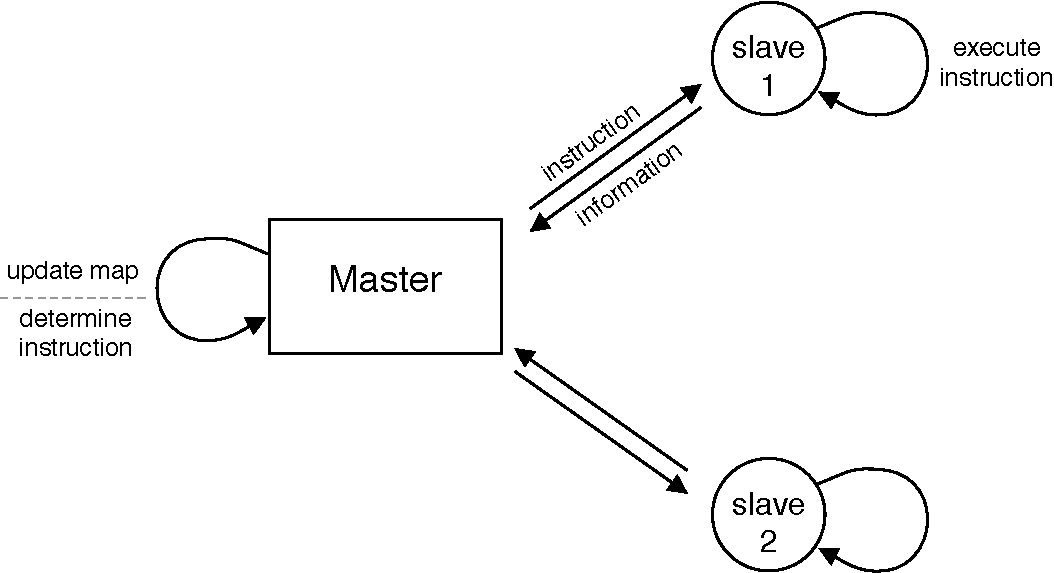
\includegraphics[scale=0.8]{figs/master-slave}
\caption{Master-slave architecture.}
\label{fig:master-slave}
\end{figure}

The next chapter describes the implementation of the master and simulator. Chapter \ref{chapter-construction} then details the construction/implementation of the physical robot. 

\chapter{Master}\label{chapter-master}

%------------------------------------------------
\section{Random environment generation}
%------------------------------------------------
The structure of the environments on which our system is tested (in the simulator and physical world) is generated randomly. The algorithm for this task had to be written from scratch since no existent one could be found. The procedure is composed of three sequential steps,
\begin{enumerate}
\item \textit{Initialization}: initialize the set of edges as shown in Figure \ref{fig:gener-a}.
\item \textit{Destruction}: remove randomly 80\%\footnote{Determined arbitrary by experimenting.} of the interior edges.
\item \textit{Fixing}: adds an edge randomly on nodes disconnected from the rest of the graph (relative to the \textit{root node}\footnote{The root node refers to the node at the bottom, and corresponds also to the starting point of the robots.}). This process is repeated until all remaining nodes can be accessed from the \textit{root node}.
\end{enumerate}

\begin{figure}[!h]
\centering
\begin{subfigure}{.3\textwidth}
  \centering
  \includegraphics[scale=0.025]{figs/complete}
  \caption{Initialization}
  \label{fig:gener-a}
\end{subfigure}%
\begin{subfigure}{.3\textwidth}
  \centering
  \includegraphics[scale=0.025]{figs/destruc}
  \caption{Destruction}
\end{subfigure}
\begin{subfigure}{.3\textwidth}
  \centering
  \includegraphics[scale=0.025]{figs/fixing}
  \caption{Fixing}
\end{subfigure}
\caption{Resulting environments of three steps of the generation.}
\label{fig:gener}
\end{figure}


%------------------------------------------------
\section{Simulator}
%------------------------------------------------
It would be costly in time to design, debug and evaluate the performance of the master algorithm if ran in combination with the physical robots. Thus, a simulator was constructed emulating environment and robots. In particular, the simulated robots are constrained to follow edges in the environment, with their sensory inputs limited to a one-step lookahead in the front, left, and right directions. Each robot increments its distance and once they encounter an intersection, an information message is send to the master.

%------------------------------------------------
\section{Communication protocol}
%------------------------------------------------
Messages are of the following form: $<$\textit{identifier}, \textit{sequence number}, \textit{message}$>$. The \textit{message} part corresponds to \textit{information} (type intersection \& distance) if the sender is a robot, or to an \textit{instruction} if it comes from the master. The \textit{identifier} is used to enable the master to distinguish robots, but also to prevent communication between the robots. Lastly, the \textit{sequence number} permits to trigger a recovery mechanism for unreceived messages and to ignore redundant messages. Delimiters ($<$, $>$) are used to verify that the entire message is received.

%------------------------------------------------
\section{Graphical User Interface}
%------------------------------------------------
Simulations are visualized in a Graphical User Interface (GUI), which was made with the framework \texttt{PyGame}\footnote{More information about the \texttt{Pygame} can be found \href{www.pygame.org}{here}.}. The GUI enables us, on the one hand to visualize the internal map representation of the master, and on the other hand the groundtruth environment and robots (see Figure \ref{fig:gui}). In order to keep the simulations smooth, the master, simulator and GUI are executed as separate threads. Let us emphasize that the same GUI is used for the physical robot exploration, but obviously does not display the groundtruth since it is not known \textit{a priori}. 

\begin{figure}[!h]
\centering
\includegraphics[scale=0.4]{figs/screen}
\caption{A snapshot of the Graphical User Interface (grey lines correspond to the groundtruth, black lines to the current internal map representation, coloured circles to the robots).}
\label{fig:gui}
\end{figure}

%------------------------------------------------
\section{Architecture \& Decision Algorithm}
%------------------------------------------------
\subsection*{Architecture}
The architecture of the master is composed of three main classes: \texttt{map}, \texttt{messenger} and \texttt{master}. When a message is send by a robot, it is received, parsed and verified by the \texttt{messenger}. The information is then passed to the \texttt{map} which updates the internal representation of the environment and the corresponding robot pose. Then, the \texttt{master} computes and sends the optimal direction that must be taken by the robot.

\subsection*{Decision Algorithm}
When a robot arrives at an intersection and sends the information, it waits for a new instruction. This instruction is determined by the decision algorithm described in the next paragraph. Beforehand, the concept of \textit{frontier}, although commonly used, must be specified: a frontier is referred to as a known but unexplored edge, i.e. the robot has sensed that there is a path but did not explore it.

The decision algorithm distinguishes three cases when a robot arrives at an intersection. In the first case, the intersection is a frontier, and thus the new direction is simply chosen by using the left-hand-rule on the unexplored edges. In the second case, the intersection is not a frontier and their are are no other frontiers in the current map. It is then concluded that the exploration is completed and the robots are send back to their start position (root note). For the last case the intersection is not a frontier, however, at least one frontier is still remaining elsewhere in the current map. The robot is then assigned to a frontier. The chose frontier is the one with the minimum Manhattan distance to the current position of the robot. Once the frontier assigned, the master computes the path to take for the robot via the $\text{A}^*$ algorithm\footnote{The Dijkstra algorithm improved with the heuristic that a path to a goal is always greater or equal to the Manhattan distance to that goal. This permits to avoid unnecessary computations. This heuristic is valid since all the angles are right.}. The robot then moves towards the assigned frontier following the determined path. However, the path is recomputed at each intersection since the explored environment expands, and thus new optimal paths could potentially be found.
 
Simulations showed that using two robots with the aforementioned algorithm increased the rapidity by 61\% compared to only using one robot. Although the results seemed sufficient, four problems appeared during the simulations. These problems are described below with a proposed solution. 

\subsection*{Avoiding robot encounters}
Since rapidity is the main objective, caution must be taken to avoid robot encounters as much as possible, since the recovery process (described in the next sub-section) would lead to a loss of time. The method applied to avoid encounters is by masking the neighbouring edges in the map around the other robot when computing a path. More specifically, the edges are masked by assigning them an infinite weight in the $\text{A}^*$ algorithm. Two cases are distinguished: if the other robot is on an intersection, the neighbourhood is defined as the set of edges directly connected to that intersection. On the other hand, if the other robot is moving on an edge, the neighbourhood corresponds to the neighbourhood of the next intersection the other robot will encounter. 

\subsection*{Handling robot encounters}
Masking the neighbourhood will not guarantee to completely avoid robot encounters. For example, two robots moving from opposite sides on an unexplored edge can not be planned/predicted. When such an encounter occurs, one of the two robots is send away, and when out of reach, the second robot updates its path and moves forward.

\subsection*{Updating assigned frontiers}
During the time a robot moves towards its assigned frontier, the other robot could potentially explore it, coming from the other side of the frontier. This issue is solved by verifying for each newly explored frontier if it was assigned.

\subsection*{Cooperative strategy}
An attempt is made to induce a cooperative behaviour. Indeed, we suggest that the exploration may be more efficient if the robots are enforced to a certain degree to explore separate distant regions. To do this, the cost function to chose the frontier is adapted as follows:
\begin{equation}
\text{cost}(\text{frontier}) = D(\text{current}, \text{frontier}) - \lambda D(\text{frontier}, \text{other robot})
\end{equation}
where the function $D$ represents the manhattan distance between two points, and $\lambda$ is the importance parameter controlling the trade-off between the two terms. The first term suggests to choose the most nearby frontier, whereas the second term induces the robot to chose the frontier which will be the most distant form the other robot.

Different values of $\lambda$ are tested, for each $\lambda$ 20 environments were generated and explored. Figure \ref{fig:coop} shows the mean elapsed time\footnote{The elapsed time rescaled by the covered length of the corresponding environment.} of the explorations. The optimal trade-off seems to be for $\lambda = 0.875$.
\begin{figure}[!h]
\centering
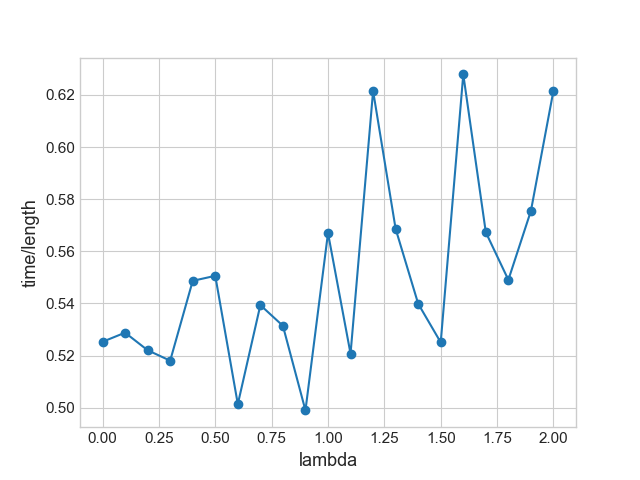
\includegraphics[scale=0.55]{figs/coop}
\caption{Mean elapsed time for different $\lambda$'s.}
\label{fig:coop}
\end{figure}

%------------------------------------------------
%------------------------------------------------
%------------------------------------------------
%\part{Robot}
%------------------------------------------------
%------------------------------------------------
%------------------------------------------------


\chapter{Robot}\label{chapter-construction}
The first part of this chapter (Section \ref{sec:components} and \ref{sec:phys-constru}) discusses physical aspects of the robot such as its components and how these are assembled. The second part then describes the software and control aspect.

%------------------------------------------------
\section{Components \& Functions}\label{sec:components}
%------------------------------------------------
We identified seven different requirements the robots needs to fulfil, they must be able to 
\begin{itemize}
\item perform basic computations.
\item move and rotate.
\item localize black lines on white background.
\item avoid collisions with the other robot.
\item measure the travelled distance.
\item communicate with the master.
\item supply power to its components.
\end{itemize}

\subsection*{Computational unit}
The \texttt{Arduino Nano} is used as the micro-controller. The main advantages are its simplicity of use and its relatively small dimensions. On the other hand, the \texttt{Arduino Nano} only contains 14 digital pins and 8 analog pins. Moreover, some capabilities (e.g. interrupt, PWM) are only available on specific pins. As a consequence of these constraints, the connectivity was a puzzle-work and the final result is shown in Figure \ref{fig:electric-diagram}.

\subsection*{Line localization}
Straightforwardly, in order to perform efficient line-following it is important to be able to localize the line with respect to the center of the robot. This problem is solved by using an infra-red (IR) reflectance sensor, which is composed of an infra-red transmitter and a photo-diode receptor. The idea is that the reflectivity of infra-red light varies with color and distance of the reflecting surface.  The transmitter emits an infra-red beam onto a surface. The surface reflects the beam which is received back at the diode. For a light-coloured surface (e.g., white background), the intensity of the reflected signal will be high, resulting in a flow of current in the diode. On the contrary, if it is dark-coloured (e.g., black line), then the intensity of the reflected signal will be low, so that the diode blocks the current. By placing an array of those sensors side-by-side, the robot becomes able to detect where the black line is positioned on the white background. 

Instead of constructing such an array from separate sensors, we use the \texttt{QTRX-MD-06A Reflectance Sensor Array}, consisting of six IR sensors (see Figure \ref{photo-bottom} in Appendix \ref{chap-construction}). In addition, it has a high-level interface permitting the robot to obtain a continuous value for the position of the line (0 if line at left extremity, 5000 if line at right extremity). A continuous value is a significant advantage since it improves the smoothness of the control system (see Section \ref{sec:line-control}). 

In practice, from this continuous value we will compute the \textit{error line}. The error line is defined as the deviation from the center, such that the center of the robot corresponds to an error of zero. Figure \ref{fig:exp-qtr-flow} shows then error for a moving black line. As can be seen, the measures do not contain significant noise, due to pre-processing steps of the \texttt{QTRX} sensor. However, it was found experimentally that shadow differences in luminous environments could affect the performance. To solve this issue a shield in carton was constructed and placed around the sensor (see Figure \ref{photo-bottom}).
\begin{figure}[!h]
\centering
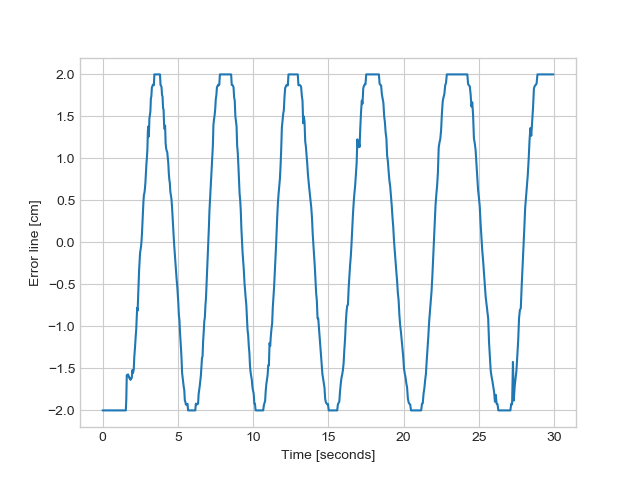
\includegraphics[scale=0.55]{figs/qtr-flow}
\caption{Experiment where a black line is moved back-and-forth between the left and right side of the robot.}
\label{fig:exp-qtr-flow}
\end{figure}

\subsection*{Obstacle detection}
Since multiple robots are moving in the environment, collisions could occur. To avoid this, a \texttt{Sharp} sensor is placed in front of the robot to detect their peers. A Sharp sensor is also an infra-red sensor but with an additional feature, it can measure the distance to an object and return a corresponding analog value. The desired behaviour is to trigger a signal quickly for an object in a range close to collision. In order to do this, we chose the \texttt{Sharp GP2Y0D805Z0F}, which detects objects between 0.5 cm and 5 cm away, and has a quick response time.

It is commonly recommended to add a bypass capacitor because the sensor draws current in large and short bursts. A bypass capacitor is a low-pass filter placed across the power and ground close to the sensor, to diminish the possible interferences resulting from these bursts.

\subsection*{Moving}
The robot is designed as a differentially steered two-wheel. It is differential in the sense that both wheels can have different rates of rotations but unlike a differential gearing system as in automobiles, a differentially steered system will have both wheels powered. In other words, to go to the left (resp. right) the speed of the right (resp. left) motor is increased. Additionally, a free rotating wheel is placed at the front of the robot to keep the body in balance and be able to rotate in both directions. Notice that the robot will rotate around the center between the two wheels. The wheels are powered by brushed DC gearmotors with a 150:1 ratio (see Figure \ref{photo-bottom} in Appendix \ref{chap-construction}), controlled by sending a special form a digital signal, namely a pulse width modulation (PWM). The higher the absolute value of the PWM, the faster the revolutions of the motor (a negative PWM corresponding to rotations in the opposite direction). In addition, a dual H-bridge \texttt{L298n} is used in order to decouple the power supply to the motors and the arduino. 

\subsection*{Distance Measurement}
The robot computes the travelled distance by multiplying speed and time, at short regular intervals. For this purpose, two quadrature encoders are soldered to the motors in order to measure the speed. The idea is that the rotating DC motors induce a hall effect in the encoders at each rotation. The used encoders trigger six counts per revolution. The number of revolutions of left and right motor, are denoted respectively $n_L$ and $n_R$. Thus, the angular velocity of the left wheel\footnote{The angular velocity of the right wheel is computed in an analogous manner.} can be computed,
\begin{equation}
w_L = 2\pi f_L
\qquad\text{with}\qquad	
f_L = \frac{n_L}{6\, G_b \, \Delta{t} }
\end{equation}
with $G_b$ the gearbox ratio, $f_L$ the rotation frequency and $\Delta{t}$ the elapsed time. The robot being modelled as differentially steered two-wheel, we obtain the speed of the robot as
\begin{equation}
v = \frac{v_L + v_R}{2} = \frac{R(w_L + w_R)}{2}
\end{equation}

with $R$ the radius of each wheel. Thus, the travelled distance is written,
\begin{align*}
\Delta{x} &= v\Delta{t}\\
&= \frac{\pi R}{6 G_b}(n_L + n_R)
\end{align*}
Several factors are not taken into account in this computation such as acceleration, noise in the measurements and the fact that the robot experiences small deviations during the line-following process. With this in mind, the computed distance is discretized in sufficiently large intervals (5 cm) to be considered completely error-free. Lastly, interrupt routines were used, since the counts of the encoders must occur independently of the program flow.

\subsection*{Communication}
Communication with the master is performed via a bluetooth module \texttt{HC-06}. This specific module is adapted for establishing short range wireless data communication between two systems. Notably, a voltage divider was added to the circuit because of the difference between the logic level voltage of the Arduino ($0-5$ Volt) and the bleutooth module ($0-3.3$ Volt) (see Figure \ref{fig:electric-diagram}).

\begin{align*} 
V_{arduino} &=  \frac{R_4}{R_3+R_4}V_{bleutooth} \\[0.4cm]
 &=  \frac{2.2}{3.2}V_{bleutooth}
\end{align*}

\subsection*{Power supply}
Most components have a low consumption. Moreover, no high-performance speed was required. Thus, a rechargeable NiMH Battery of 7.2 Volts with a capacity of 900 mAh seemed sufficient.

%------------------------------------------------
\section{Physical construction}\label{sec:phys-constru}
%------------------------------------------------
The robot is constructed following the steps described below:
\begin{enumerate}
\item A chassis is cut from wood and used as a base. Additionally, four small pillars are pasted at the corners (see Figure \ref{photo-chassis} in Appendix \ref{chap-construction}).
\item The H-bridge is screwed on the chassis.
\item A breadboard is pasted on the pillars.
\item The micro-controller is soldered into header pins which are then fixed in the breadboard.
\item The encoders are soldered to the motors, and the latter are then fixed on the bottom of the chassis.
\item The wheels are placed on the shafts of the motors, and the omni-wheel is placed under the chassis, at the front.
\item The Sharp and QTR sensor along with its shields are fixed at their desired place.
\item Wiring all the components (see Figure \ref{fig:electric-diagram}).
\item Connect to the power via a soldered switch.
\end{enumerate}

\clearpage
\vfill
\begin{figure}[!h]
\centering
\includegraphics[scale=0.9]{figs/electric-diagram}
\caption{Electric diagram of the robot}
\label{fig:electric-diagram}
\end{figure}
\vfill
\clearpage

\section{High-level algorithm}\label{sec:high-algo}
The main steps of the robot's algorithm are detailed below. As can be observed, the robot executes mostly physical operations whereas the Master does all the 'smart' stuff.

\begin{algorithm}
    \caption{High-level view algorithm robot}
    \label{euclid}
    \begin{algorithmic}[1] % The number tells where the line numbering should start
    		\Procedure{main}{} 
    			\State active $\gets$ False
    			\State distance $\gets$ 0
			 \While{True}
			 	\If{\Call{checkMessage}{}}
					\State instruction $\gets$ \Call{readMessage}{}  
					\If{instruction $== 0$}
						\State \Call{stopMotors}{}
						\State active $\gets$ False
					\Else
						\State \Call{execInstruction}{instruction} \Comment{turn left, turn right, uturn}
						\State active $\gets$ True
					\EndIf
				\EndIf
				\If{active}
					\State \Call{followLine}{}
					\State distance $\gets$ \Call{measureDistance}{} + distance
					\If{\Call{isIntersection}{}} \Comment{see subsection below}
						\State type $\gets$ \Call{classifyIntersection}{} \Comment{see subsection below}
						\State \Call{forwardAlign}{} \Comment{see subsection below}
						\State \Call{send}{distance, type} \Comment{to Master}
						\State active $\gets$ False
					\EndIf
				\EndIf
				\State \Call{wait}{20} \Comment{milliseconds}
			 \EndWhile        		
        \EndProcedure
    \end{algorithmic}
\end{algorithm}

\subsection*{Intersection detection \& classification}
An anomaly is triggered when black is detected at one of the extremities of the \texttt{QTR} sensor. Since it could be a noisy measure, the robot continues its execution and checks if the same anomaly pattern occurs consecutively. If this is the case, the anomaly is finally viewed as an intersection. Whenever an intersection is detected, it continues its movement for a few inches in order to classify its type as given by Figure \ref{fig:types}.

\begin{figure}[!h]
\centering
\includegraphics[scale=0.55]{figs/type-intersections}
\caption{Different types of intersections.)}
\label{fig:types}
\end{figure}

\subsection*{Forward align}
Since the robot rotates around the central point between the wheels (at the back), the robot must align the wheels with the detected intersection. This permits the robot to still be nicely aligned after a turn, and thus avoid large initial deviations in the line-following. In other words, once an intersection is detected the robot moves forward for a distance equivalent to its own length. As there may be no black line in front, the robot moves without the follow-line procedure but instead controls the speed of the two motors to be equal in order to go in a straight line.

\section{Architecture}\label{sec:archi}
Figure \ref{fig:architecture} shows the architecture of the implementation in the micro-controller. The \textit{main} corresponds to the algorithm above. The \textit{COEX} class refers to the high-level features related to the cooperative exploration, which is based on low-level features. The advantages offered by this modularity are two-fold: it makes the debugging easier and the low-level features could be re-used for a different purpose.

A particular problem observed experimentally was that the sensors and actuators had optimal performance at different frequencies. The solution implemented assigns a frequency object to each to component/task.

\begin{figure}[!h]
\centering
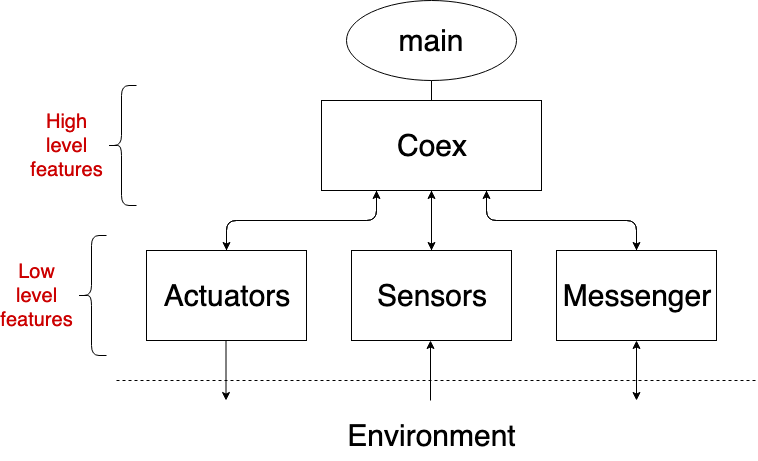
\includegraphics[scale=0.3]{figs/architecture}
\caption{Architecture of the code of the robot.}
\label{fig:architecture}
\end{figure}


%------------------------------------------------
\section{Control}
%------------------------------------------------
\subsection*{Line Following \& Speed Control}\label{sec:line-control}
As a beginner roboticist I thought naively that the robot would go straight if the signal (PWM) send to the left and right motor were equal. To verify that this claim does not hold in reality, an experiment was performed were the same PWM signal is send to both motors and their respective speed are measured with the encoders. The result is shown in Figure \ref{fig:probs-control}. A varying difference between the two motors can clearly be noted. Moreover, we also observe that this relationship varies as the power supply discharges. With this in  mind a speed controller was developed in addition to a line-following controller. The two controllers take the form of a PID and are combined as in Figure \ref{fig:control-base}. Straightforwardly, the error of the speed controller is the \textit{target speed}\footnote{For the demo we fix the target speed to 8 centimeter per second.} $v^*$ minus the \textit{measured speed} $v$. On the other hand, the error of the direction controller is given by the so-called \textit{error line}, $x^*-x$ (previously discussed in Section \ref{sec:components}). The computed PWM values are denoted $u_L$ and $u_R$ for the left and right motor. With anti-windup.
\begin{figure}[!h]
  \centering
  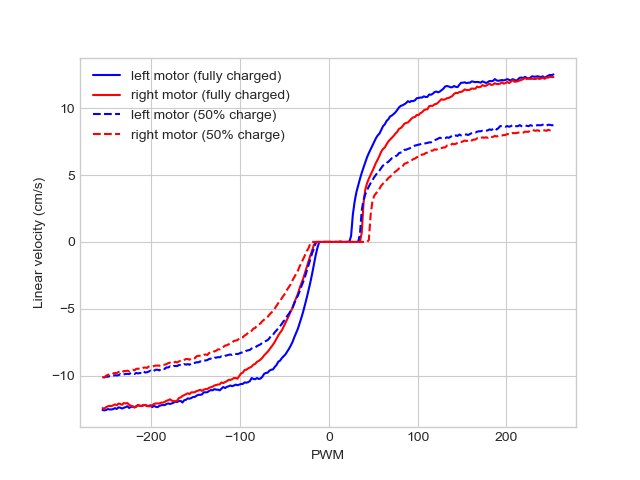
\includegraphics[scale=0.6]{figs/motors_merged}
\caption{Variations of speed between the motors}
\label{fig:probs-control}
\end{figure}

The tuning of the parameters of the speed controller is done with respect to a target speed varying as in Figure \ref{fig:tuning}. Notice that the measured speed in this Figure is the one obtained using the tuned parameters. The speed controller seems to work but there is still some room for improvements. However, the results were sufficient for our purpose and thus no further tuning was applied. 
\begin{figure}[!h]
\centering
\begin{subfigure}{.5\textwidth}
  \centering
  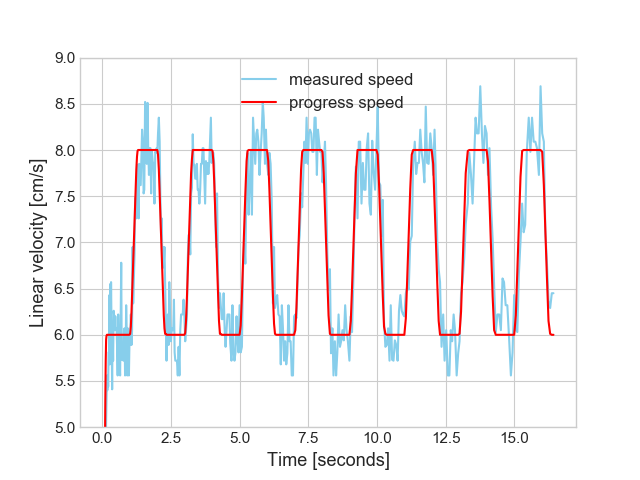
\includegraphics[width=\linewidth]{figs/pid_speed_normal}
  \caption{multiple cycles}
\end{subfigure}%
\begin{subfigure}{.5\textwidth}
  \centering
  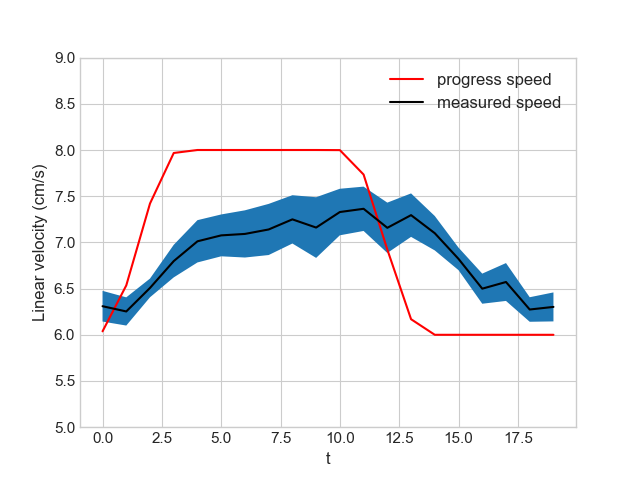
\includegraphics[width=\linewidth]{figs/pid_speed_shaded}
  \caption{average trend with bandwith representing the variance}
\end{subfigure}
\caption{Experiment speed control with a varying target speed}
\label{fig:tuning}
\end{figure}

To adjust the parameters of the direction controller, the robot was placed on a parcours formed by curved black lines. The heuristic used for tuning was to double the $K_p$ parameter until oscillations occurred, then half it back one time and start to tune the other parameters. Once this was done, the target speed was increased by a small increment and the process repeated (until the desired behaviour). 

By experimenting, several improvements were developed as can be viewed in the block diagram of Figure \ref{fig:control-base}. Indeed, the first observation to make is that there are a lot starts/stops during the exploration, which caused instabilities. It was suspected that this was due to a high current drainage by the motors for a sudden acceleration. A solution is to design and implement a smoother acceleration profile\footnote{See Appendix \ref{chap-extra}.} for a desired target speed to attain in a specific time interval, an intermediate value is computed namely the \textit{progress speed} The progress speed follows an acceleration in trapezoidal form, permitting the robots to have a slower start. 



Another challenge is that there can be a misalignment between the black line and the center of the robot after a turn. As a result, a \textit{derivative kick}\footnote{A derivative kick refers to a very large derivative as a consequence of a significant error. As large corrections are undesired, a common approach is to derive the measurements instead (already our case by default since setpoint remains unchanged) and to fix initial derivation to zero.} can occur, which was solved by fixing the initial derivation to zero. A second consequence of the misalignment is that in combination with the smooth acceleration, the correction from the direction controller is potentially too large with respect to the correction of the speed controller. This issue was solved by having a dynamic setpoint weighting, so that the direction correction is weighted with an hyperbolic tangent function converging rapidly with time to unity. 

\subsection*{Turning}
The COEX-1 is modelled as a two-wheel robot (see figure below). By integrating the angular velocity under the assumption that $v_R = -v_L$, rotational displacement can be deduced
\begin{equation}\label{eq:theta-turn}
\theta(t) = \frac{2vt}{b} + \theta_0
\end{equation}
\begin{figure}[hbtp]
\centering
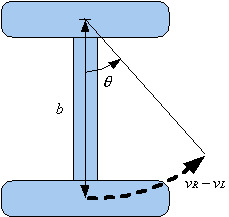
\includegraphics[scale=0.45]{figs/differential-system}
\caption{Rotation of COEX-1}
\label{fig:model-turn}
\end{figure}

In order to rotate in a specific direction, a naive approach was first tested: rotating at a given speed and duration to obtain the desired angle using Equation \ref{eq:theta-turn}. The results were not catastrophic, but a significant variance was observed, going from a few degrees to a few dozens. This is not acceptable as our goal is to have the center of the robot aligned as closely as possible to the black line. 

A second approach tested, was to use \texttt{QTR} sensors to detect when the line was in the middle and at that instant, to stop the robot. Notice that if the the robot needs to turn 180 degrees but if edges are at his sides (90 degrees), the robot will stop to soon. To this end, the robot was first rotated with an angle of 130 degrees (using the method of the previous paragraph) and then continued with the \texttt{QTR} solution until the robot is aligned. An improvement was observed, however, the robot always stopped a little too late due to drift of the wheels with the surface and a lack of response time from the sensors/actuators.

Ideally, the robot would decrease its rotation speed when approaching the line and sufficiently slow to stop and be aligned perfectly. The implemented solution uses a simple controller so that the speed is decreased with respect to the error line measured. The deceleration was triggered from the moment the black line was in the range of the sensor (i.e., at one of its extremities).

\newpage
\null
\vfill
\begin{figure}[!h]
\centering
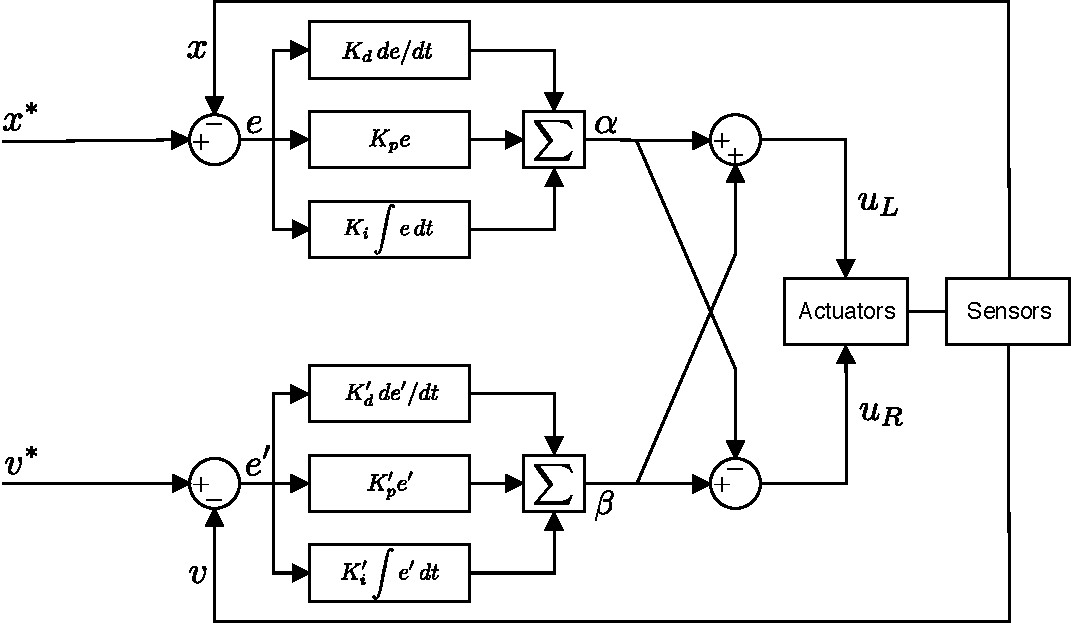
\includegraphics[scale=0.85]{figs/control-base}
\caption{Schematic diagram of the control system (with anti-windup).}
\label{fig:control-base}
\end{figure}
\vfill
\begin{figure}[!h]
\centering
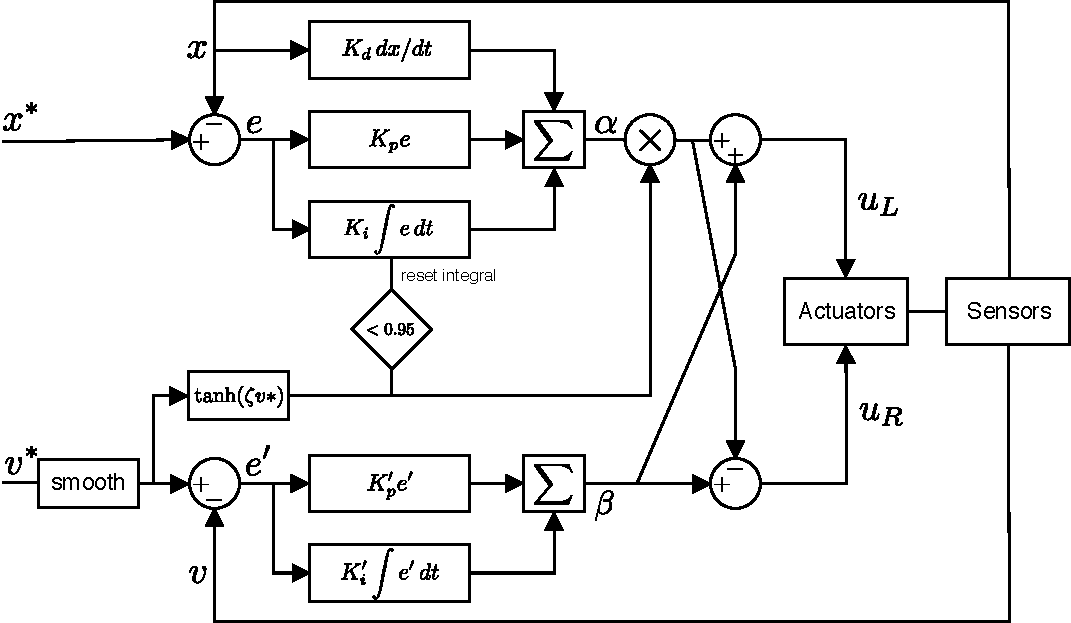
\includegraphics[scale=0.85]{figs/control-improve}
\caption{Schematic diagram of the improved control system (with anti-windup).}
\label{fig:control-base}
\end{figure}
\clearpage
\newpage






%------------------------------------------------
%------------------------------------------------
%------------------------------------------------
%\part{Result}
%------------------------------------------------
%------------------------------------------------
%------------------------------------------------


\chapter{Conclusion}\label{conclusion}
The algorithm of the master that was developed in simulation, showed satisfying results. We verified an improvement from using two robots instead of one. In addition, a slight performance gain was illustrated by inducing a simple cooperative behaviour, enforcing the robots to explore distant regions to a certain degree.

Constructing and implementing the physical robot to be robust and fast was challenging. Nevertheless, an efficient error-free mapping system with one robot could be demonstrated.

Finally, two robots were used to map a physical environment. No entirely error-free solution was found as collisions could not be avoided for certain angles and speeds.




%------------------------------------------------
%------------------------------------------------
\newpage
\appendix
\chapter{Smooth acceleration}\label{chap-extra}
The default acceleration profile is uniform (see Figure \ref{fig:a}). The update of the progress speed is as follows
\begin{align*}
&v_{n+1} \leftarrow v_n + A \, \Delta t_{n:n+1}\\
&\text{with}\,\ A = \frac{v_{target}}{T}
\end{align*}
For a smoother transition, the robot accelerates following the trapezoidal profile as in Fig.\ref{fig:b}. As we want the robot to achieve the target speed in the same amount of time $T$. This constraint is developed,
\begin{align*}
&\Leftrightarrow \int_{0}^{T}a(t) =  \int_{0}^{T}a'(t) \\
&\Leftrightarrow A\,T = \underbrace{d\,B}_{triangles} + \underbrace{(T - 2d)B}_{rectangle}
\end{align*}
\begin{figure}[!h]
\centering
\begin{subfigure}{.5\textwidth}
  \centering
  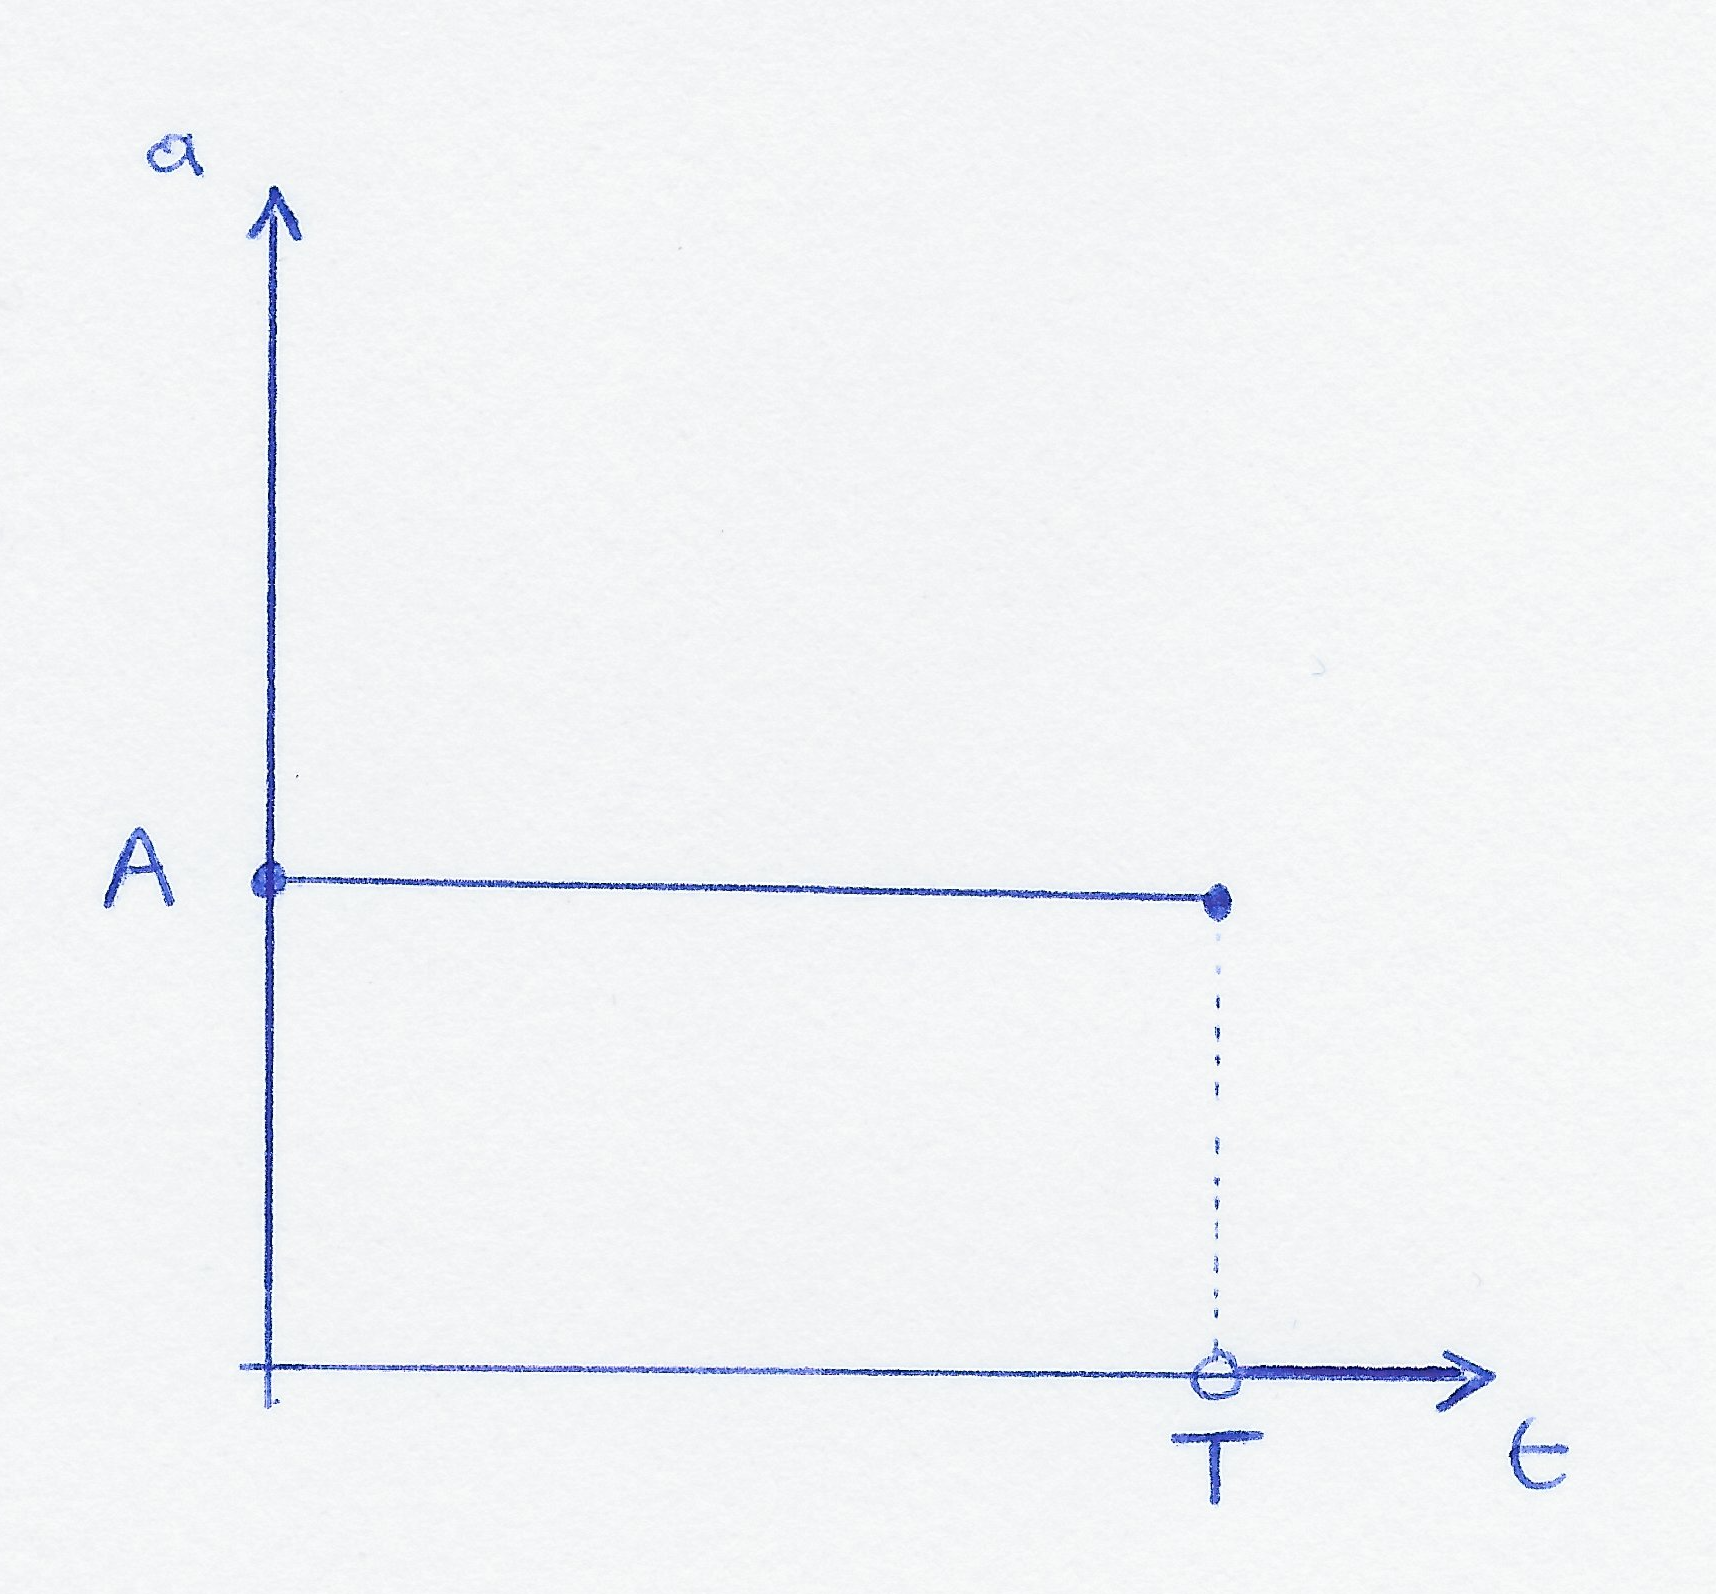
\includegraphics[width=\linewidth]{figs/uniform-acc}
  \caption{uniform}
  \label{fig:a}
\end{subfigure}%
\begin{subfigure}{.5\textwidth}
  \centering
  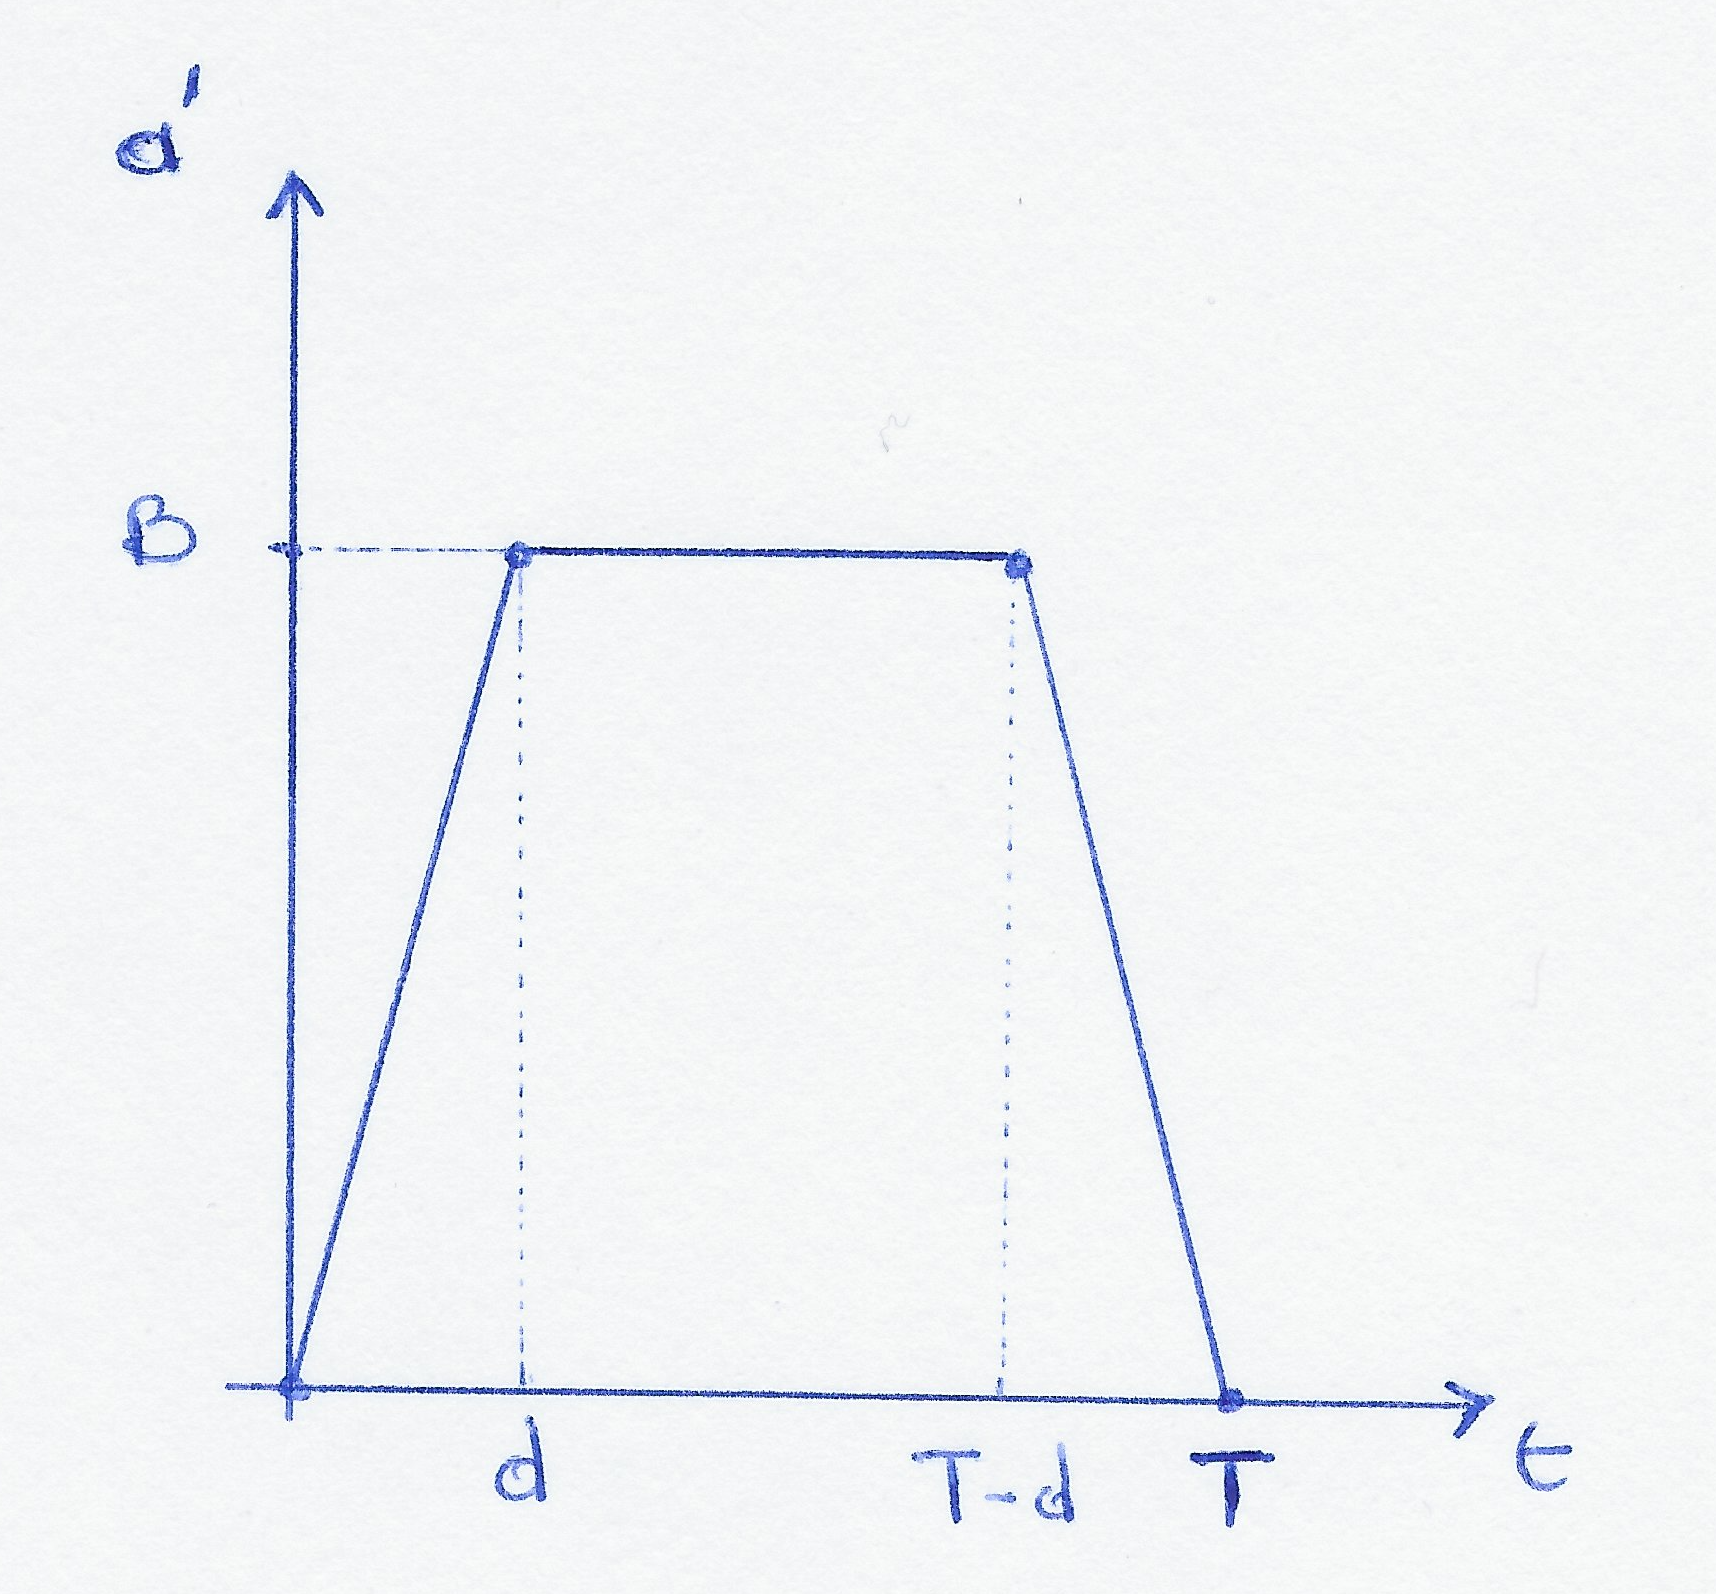
\includegraphics[width=\linewidth]{figs/smooth-acc}
  \caption{trapezoidal}
  \label{fig:b}
\end{subfigure}
\caption{Acceleration profiles.}
\label{fig:ab}
\end{figure}
By substituting the parameter $\psi = \frac{d}{T}$, we obtain
$$
\boxed{B = \frac{A}{1-\psi}} 
$$
The update rule for the progress speed becomes
$$
v_{n+1} \leftarrow v_n + \int_{n}^{n+1}a'(t) = v_n + \int_{0}^{n+1}a'(t) - \int_{0}^{n}a'(t)
$$
Notice that with the right hand side of the above expression, we can make use of precomputed values of the geometric surfaces.
\chapter{Construction}\label{chap-construction}

\begin{figure}[hbtp]
\centering
\hspace*{-1.8cm}\begin{tikzpicture}
	\node [anchor=west] (bluetooth) at (-1.95,5) {\small Bluetooth};
	\node [anchor=west] (nano) at (-1.6,3) {\small Nano};
	\node [anchor=west] (sharp) at (-1.6,1) {\small Sharp};
	\node[anchor=south west,inner sep=0] (image) at (0,0) {\includegraphics[scale=0.28]{figs/img_front}};
	\begin{scope}[x={(image.south east)},y={(image.north west)}]
		%\draw[help lines,xstep=.1,ystep=.1] (0,0) grid (1,1);
		\draw[yellow,ultra thick,rounded corners] (0.62,0.25) rectangle (0.72,0.40);
		\draw[yellow,ultra thick,rounded corners] (0.35,0.60) rectangle (0.45,0.83);
		\draw[yellow,ultra thick,rounded corners, rotate around={48:(0.55,0.50)}] (0.55,0.50) rectangle (0.65,0.70);
		\draw [-latex, ultra thick, yellow] (bluetooth) to[out=0, in=-120] (0.35,0.6);
		\draw [-latex, ultra thick, yellow] (nano) to[out=0, in=-120] (0.5,0.55);
		\draw [-latex, ultra thick, yellow] (sharp) to[out=0, in=-160] (0.62,0.32);
	\end{scope}
\end{tikzpicture}
\caption{Front view of robot}
\label{photo-top}
\end{figure}

\begin{figure}[hbtp]
\centering
\hspace*{-1.5cm}\begin{tikzpicture}
	\node [anchor=west] (battery) at (-1.6,5) {\small Battery};
	\node [anchor=west] (shield) at (-1.6,3) {\small Shield};
	\node[anchor=south west,inner sep=0] (image) at (0,0) {\includegraphics[scale=0.28]{figs/img_side.JPG}};
	\begin{scope}[x={(image.south east)},y={(image.north west)}]
		%\draw[help lines,xstep=.1,ystep=.1] (0,0) grid (1,1);
		\draw[yellow,ultra thick,rounded corners] (0.65,0.35) rectangle (0.75,0.62);
		\draw[yellow,ultra thick,rounded corners] (0.38,0.23) rectangle (0.55,0.35);
		\draw [-latex, ultra thick, yellow] (battery) to[out=0, in=120] (0.65,0.62);
		\draw [-latex, ultra thick, yellow] (shield) to[out=0, in=-120] (0.38,0.23);
	\end{scope}
\end{tikzpicture}
\caption{Side view of robot}
\label{photo-side}
\end{figure}

\begin{figure}[hbtp]
\centering
\hspace*{-2.6cm}\begin{tikzpicture}
	\node [anchor=west] (array) at (-3.5,5) {\small Reflectance array};
	\node [anchor=west] (motors) at (-1.6,3) {\small Motors};
	\node[anchor=south west,inner sep=0] (image) at (0,0) {\includegraphics[scale=0.28]{figs/img_bottom.JPG}};
	\begin{scope}[x={(image.south east)},y={(image.north west)}]
		%\draw[help lines,xstep=.1,ystep=.1] (0,0) grid (1,1);
		\draw[yellow,ultra thick,rounded corners] (0.47,0.5) rectangle (0.68,0.65);
		\draw[yellow,ultra thick,rounded corners] (0.38,0.11) rectangle (0.75,0.25);
		\draw [-latex, ultra thick, yellow] (array) to[out=0, in=120] (0.47,0.65);
		\draw [-latex, ultra thick, yellow] (motors) to[out=0, in=150] (0.55,0.25);
	\end{scope}
\end{tikzpicture}
\caption{Bottom view of robot}
\label{photo-bottom}
\end{figure}

\begin{figure}[hbtp]
\centering
\hspace*{0.85cm}\includegraphics[scale=0.28]{figs/chassis}
\caption{Wooden chassis}
\label{photo-chassis}
\end{figure}



%\chapter{Algorithms}
%...

%\chapter{Miscellaneous}
%...

%------------------------------------------------
%------------------------------------------------
\bibliographystyle{plain}
\bibliography{biblio}

\end{document}
